\begin{center}
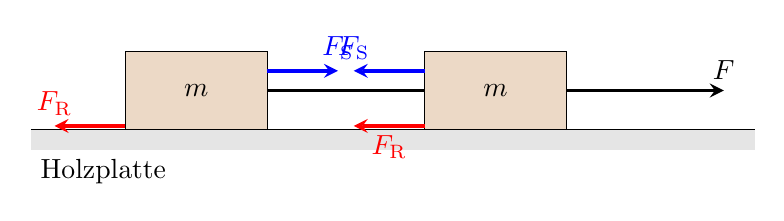
\begin{tikzpicture}[>=stealth]
 \fill[gray!20] (-4.6,0) rectangle (4.6,-0.25);
 \draw (-4.6,0) -- (4.6,0);
 \node[anchor=north west] at (-4.6,-0.25) {Holzplatte};
 \draw[fill=brown!30] (-3.4,0) rectangle (-1.6,1);
 \draw[fill=brown!30] (0.4,0) rectangle (2.2,1);
 \draw[thick] (-1.6,0.5) -- (0.4,0.5);
 \node at (-2.5,0.5) {$m$};
 \node at (1.3,0.5) {$m$};
 \draw[->, very thick] (2.2,0.5) -- ++(2,0) node[above] {$F$};
 \draw[->, very thick, blue] (-1.6,0.75) -- ++(0.9,0) node[above] {$F_\mathrm{S}$};
 \draw[->, very thick, blue] (0.4,0.75) -- ++(-0.9,0) node[above] {$F_\mathrm{S}$};
 \draw[->, very thick, red] (-3.4,0.05) -- ++(-0.9,0) node[above] {$F_\mathrm{R}$};
 \draw[->, very thick, red] (0.4,0.05) -- ++(-0.9,0);
 \node[red, anchor=north] at (-0.05,0.05) {$F_\mathrm{R}$};
\end{tikzpicture}
\end{center}

Für Holz auf Holz ist $\mu_\mathrm{G} = \muGO$ (FoTaBe S.~189). Auf jeden Klotz wirkt die Gleitreibungskraft $\mu_\mathrm{G}\,m\,g$. Für beide Klötze zusammen (Masse $2m$) gilt nach dem Aktionsprinzip
\begin{align}
 F - 2\,\mu_\mathrm{G}\,m\,g &= 2m\,a
\end{align}
und damit
\begin{align}
 a &= \aHkF \\
   &= \frac{\FZu}{2\cdot\mHk}-\muG\cdot\gE \\
   &= \aHk \approx \result{\aHkP{0}{2}}
\end{align}
Die Schnur zieht nur am hinteren Klotz nach vorne:
\begin{align}
 F_\mathrm{S} - \mu_\mathrm{G}\,m\,g &= m\,a \quad\Rightarrow\quad F_\mathrm{S} = m\left(a+\mu_\mathrm{G}\,g\right) = m\cdot\frac{F}{2m}
\end{align}
also
\begin{align}
 F_\mathrm{S} &= \FSnF = \frac{\FZu}{2} = \result{\FSnP{0}{3}}
\end{align}
Die Schnurkraft ist unabhängig von der Reibungszahl, die Beschleunigung dagegen hängt stark vom unsicheren Wert $\mu_\mathrm{G} = \muGO\pm\dmuO$ ab.
